\documentclass[emulatestandardclasses]{scrartcl}
\usepackage{graphicx}
\usepackage{color}
\usepackage[ngerman]{babel}
\usepackage{hyperref}
\usepackage{fullpage}
\usepackage{calc} 
\usepackage{enumitem}
\usepackage{titlesec}
\newcommand{\todo}[1]{\textcolor{red}{TODO: #1}\PackageWarning{TODO:}{#1!}}
\date{\vspace{-3ex}}
\begin{document}

\title{
	\includegraphics*[width=0.75\textwidth]{ErstesSem/images/hu_logo.png}\\
	\vspace{24pt}
	Maps of Meaning}
\subtitle{Lecture 2016\\
          Jordan B. Peterson\\
          University of Toronto}
\author{Lennard Wolf\\
        \small{\href{mailto:lennard.wolf@student.hu-berlin.de}{lennard.wolf@student.hu-berlin.de}}}
\maketitle
\begin{abstract}

Maps of Meaning is a university course taught by Dr. Jordan B Peterson. It describes how the world is portrayed in story form in myths, rituals and religious conceptualizations and how that is related to brain function and behavior. In doing so, it presents a solid alternative to nihilism and totalitarianism. 

\end{abstract}
\newpage

\tableofcontents
\listoffigures
\newpage


\section{Introduction\\(30.04.17)}

\subsection{Classwork - Selfauthoring}

\begin{itemize}
  \item Uncertainty is extremely stressful to the body, like a real danger at the moment
  \item Writing about the past (difficult, hard to understand) is extremely helpful in overcoming this stress
  \item Divide life in to 7 epochs: What happened there?
  \item Memory is for learning and doing things better in the future, but it has to be actively employed in this way 
\end{itemize}

\subsection{Motivation}

\begin{itemize}
  \item In cold war, most people around Dr. Peterson thought that we were not going to see the 21st century, which made them ask 'Whats the point?' and act nihilistically
  \item Dostoyewski the one thing you can say about human history is that its not raational
  \item Fire as purifying agent: Hitler, Stalin were maybe not in for the win, but for the fire. The Columbine kids were not in to win, their suicide especially makes that point. (Note: Its very naive to think they did that because they were bullied. Most people are outcasts, they would not even \emph{think} about killing someone because of that, let alone kill dozens of people and yourself)
  \item How could it be that the world would divide into two hyper aggressive, hateful, armed camps, with tens of thousands of nuclear weapons, enough to destroy each other multiple times? (see "`MAD"', mutually assured destruction program) Why were both sides entirely convinced that \emph{they} were right? Were both wrong? Were both right?
  \item If both are right/wrong, none of them: What does that mean? If one side is right in defending their principles, in what would these principles be grounded?
  \item Goal of lecture: Why do people believe the things they believe? What is Malevolence? (Difference between morally wrong and evil) 
  \item Rousseau vs Hobbes: People are good (but why do chimpanzees go to war?) vs People are bad and have to be constrained by institutions
  \item chimpanzees go to war, they have no control over their aggressions! Why are we so sure that we are in control of our aggressions? Chimpanzees keep each other in control through fear of each other
  \item Human tribes think a lot about other tribes, the tend to call themselves "`the people"', or "`the human beings"' (not necessarily literally), making the others unhuman/barbarian (people that talk like "`bar bar bar"')
  \item What humans have that animals dont: I know how I can hurt you because I know how I can be hurt. We are thus \emph{very} powerful.
  \item THUS we can not afford to not understand/have control over our (subconcsious) malevolence!
\end{itemize}

\subsection{Main problems discussed in this lecture series}

\begin{itemize}
  \item Not a sociological/political problem: Marxists are right in a way, that the control of that which is of value defines everything about the conditions of society. But Peterson thinks we need to take a more fundamental approach, which is understanding what actually constitutes \emph{value} - and value is not universal, its intrinsically cultural (oil is only a basic value if you own a car), except maybe air and water. Peterson also maintains that all motivation is not economic, its psychological, e.g. dominance in a hierarchy etc - economic power is just this cultures (?) way of being on top of the food chain, making women more attracted to men so that they can procreate on a higher scale. Economics thus is only a secondary consequence.
  \item Anecdote: Young males become hyper aggressive in situations where they can not win.
  \item Anecdote: Quebec became secular in 60s, before that they were Catholics with families of about 12 people, after that they got to the lowest brith rate on earth, and became nationalist/separatist. Good example of how one belief was just exchanged for another.
  \item Usually people act morally because they are too afraid to act immorally and thus are able to just say they are moral, which they aren't because they would if only they were brave enough. Nietzsche didn't say morality is cowardice, but that cowardice acts as morality.
  \item In discussions, people tend to create caricatures of the others in their and blast them (strawman), which is pathetic. Instead they should help the other state their case as best as they can, and then they should see whether they are still right above the other. Only then can discussions go somewhere.
  \item Why did the chicken cross the road? Because it thought the other side was better! Action only comes from the belief that it is more valuable to do something that not doing it. So everybody who does something and doesn't just sit around believes \emph{something}
  \item Problem Peterson struggled with: You cannot not have a belief system, but if people have belief systems (which inevitably differ), they cannot not fight!
  \item Next goals of lecture: Why do people have belief system? What are belief systems? What can you do if people around you have a different belief system than you? What patterns underly the process under which belief systems are modified and negotiated so that belief systems that have different structures can coexist in the same place peacefully? This question is important because we only have 3 options: Being a slave, a tyrant, or a negotiator, and the last is the hardest, but the best. (You have to listen to your enemy, because the only other option is fighting them)
  \item When looking at ideologues, it is important to ask what they are \emph{against}, not what they are for, because they think that the right is on their side, which makes them susceptible to ignoring their shadow (Jungian perspective). "`Yeah yeah, thats what you're for, sure, but I know that negative motivations are more powerful than positive ones."'
  \item Orwell critique of socialists: Of course we have to help the poor lower class coal miners, but thats, in his experience, not the main concern of the socialists. Their main concern is with the "`rich"' people and full of resentment and anger, instead of benevolence!
  \item Psychoanalyst approach: If you say, "`Here is how I am positively predisposed."', the psychoanalyst says: how are you using that to mask something easy and malevolent that youre doing? $\rightarrow$ Be bloody weary of people who do too much for you! (The witch gives food to Hansel and Gretel to eat them later - overly nice and protective parents will never want to let go of their children, they want to possess them, and in turn the children will feel useless themselves, because everything iss done for them)
  \item Dealing with children/elderly: You steal from them if you take away their obstacles!
 \end{itemize}

\begin{figure}[h]
	\centering
	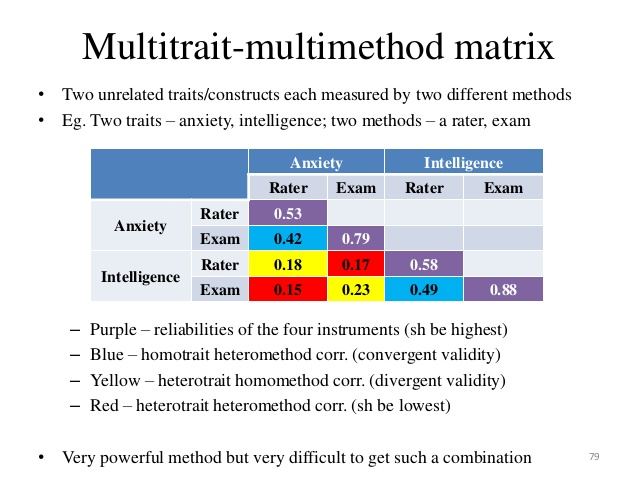
\includegraphics[width=0.75\textwidth]{images/mmm}
	\caption{Multi-Method Matrix}
	\label{fig:mmm}
\end{figure}

\subsection{Truth and meaning}

\begin{itemize}
 \item How do you know if something is true so that you can use it as a foundation of your belief system? By constantly chipping away at it and questioning it so that it can never be broken from the outside! 
  \item Pragmatic definition of truth: You don't know anything, but if something is true enough for a particular function, then it suffices. If you undertake an action, you always implicitly show a predictive theory about that action and the circumstances surrounding it. "`This is true enough if what I predict will happen happens."' | This is great, because we always will only have partial knowledge and not be omniscient, but at least we can work with it.
  \item The stories that are at the basis of our culture are pragmatic truths! 
  \item It does not suffice that we know what the world is made up of, but what to do with that knowledge! And exactly that can never be objectively true, but only pragmatically! People confuse the "`fact"' that science is value free with the idea that life is value free. 
  \item When you ask whether something exists (e.g. anger), it tends to be very hard to extract that exact thing out of where it occurs (e.g. a speech) and the accompanying context $\rightarrow$ If you want to proof something exists you have to do so using \emph{different methods} $\rightarrow$ Multi-Method Matrix (Example on our selves: We have multiple senses to verify the contents of our surroundings in various ways!)
  \item People have the feeling that something of truth has been revealed, when they find a pattern that underlies certain phenomena that (they think) are related. (these patterns might actually just be due to too narrow observation) Or: a decrease in entropy, and if that newly observed pattern actually reaches over many many previously unrelated phenomena, then people have what some might call a "`spiritual awakening"'
  \item Peterson: "`Apparently I never tell anyone anything they don't already know, probably because of the archetypal structures that are touched"'
  \item Debatable presupposition of science: "`the world is an objective place because we can describe it objectively"', but it misses the point of subjective experience, which puts meaning into things and is actually the basis of everything about us as humans. Furthermore, humanity has survived without science quite well for most of the time, the scientific method is rather new, and might just be a better way of advancing tools, but it does not really help us in understanding the workings of ourselves, human interaction, society, or humanity as a whole, which is way more directly related to our overall experience of life.
  \item Science started as a tool to further the \emph{moral} project of the enlightenment, but happened to sort of be outside of that sphere too
  \item It helps to look at theories of reality as \emph{tools} instead of \emph{descriptions}, because then you don't have to think of one as \emph{better}, but rather as more useful in the pragmatic sense of truth.
  \item One can make better assumptions about a person through their behavior than their words
  \item Saying that morality does not exist is certainly true from the viewpoint of materialism, but engaging with a topic from just one standpoint is radically reductionist and ignorant, as in the end it is just a viewpoint (anschauung), which can in turn can only create a model, and never the thing itself, so it will always be lacking!
  \item How do we find the meaning within an essay? We have meaning within letters, words, sentences, sentence structures, paragraphs and so on. On all of these levels an understanding has to exist, and so on all of these levels there can be mistakes (bad spelling, words used in a wrong way, unclear sentence structure). But the meaning really isnt in the essay but in the shared cultural context, or even worse, the cultural context itself is nested in a historical framework, or even a biological framework or even ... ad infinitum. So the meaning of the essay is not something to be \emph{found} somewhere, but rather an interplay of an infinity of factors, including subjective experience.
  \item So if we talk abou "`the essay"', "`the song"', what are we talking about? The words? the Notes? Anything that we talk about is fundamentally tied, relational, to us
  \item From this observation we can understand the complexity of \emph{any} statement, which is basically full of layers and layers of meaning. It would be quite easy from this point to jump to any sort of relativism concerning meaning, for example moral relativism.
  \item Example: What if in Monopoly everybody could steal each others' hotels at any point in time. Would people want to play that? Why not? Why would that be a stupid game? Because of the chaotic nature? because there would be no end? No purpose in doing anything?
  \item Games are like moral systems.
\end{itemize}







\begin{description}[leftmargin=!,labelwidth=\widthof{\bfseries Transzendentalphilosophie bei Kant}]
  \item[] 
\end{description}



\newpage
\section{"Uber den Professor}
Prof. Mustermann ist..


%\begin{figure}[h]
%	\centering
%	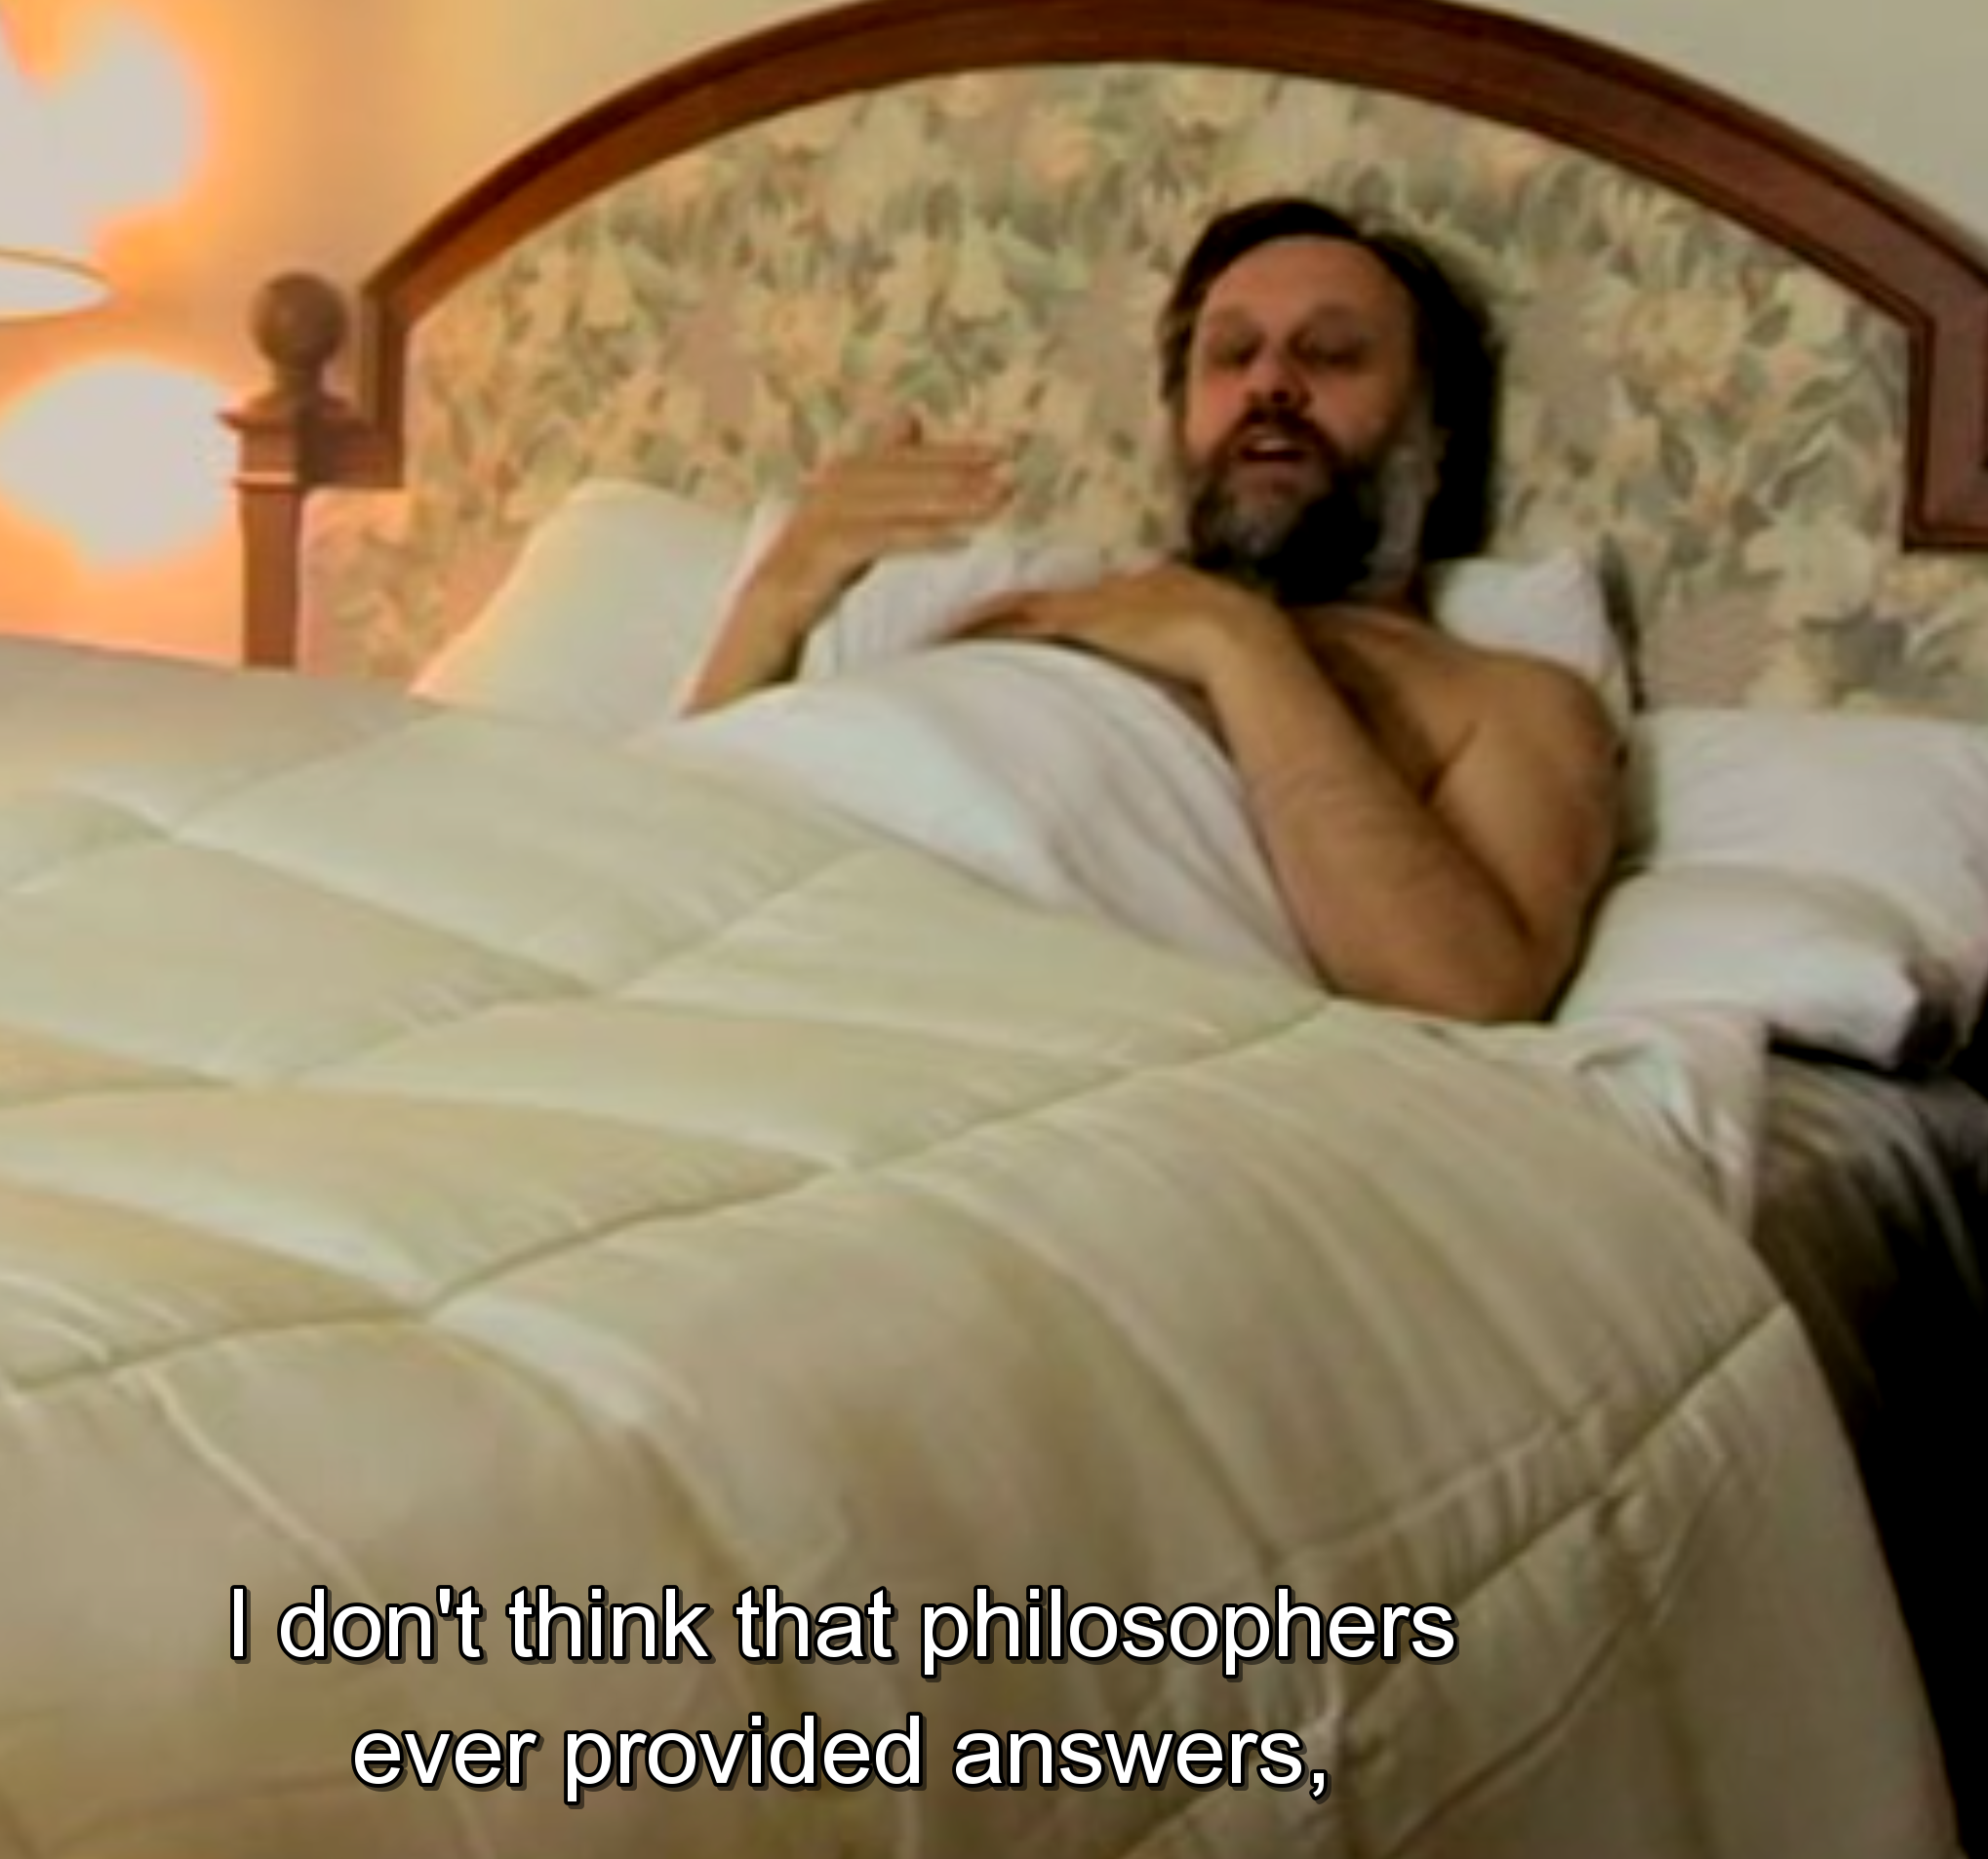
\includegraphics[width=0.5\textwidth]{images/template.png}
%	\caption{Template Bild}
%	\label{fig:template}
%\end{figure}

\end{document}
